In the following we introduce an alternative way of defining the canonical form for isometric tensor product states, which has some important differences to the isoTPS discussed in Section \ref{sec:tensors_and_tensor_networks_isometric_tensor_product_states_in_2D}. We start by introducing this canonical form in Section \ref{sec:YB_isoTPS_network_structure}. To move the orthogonality hypersurface, a new algorithm must be implemented, which we call the \textit{Yang-Baxter} (YB) move and discuss in Section \ref{sec:YB_isoTPS_yang_baxter_move}. Finally, in Section \ref{sec:YB_isoTPS_TEBD} we generalize the TEBD algorithm to this new canonical form.

\section{Network Structure}
\label{sec:YB_isoTPS_network_structure}
\documentclass[crop,tikz,convert={outext=.svg,command=\unexpanded{pdf2svg \infile\space\outfile}},multi=false]{standalone}
% This file is used to globally define colors, line widths, etc. for diagrams used in the thesis
\usepackage{tikz}
\usepackage{ifthen}

% Libraries
\usetikzlibrary{decorations.markings}
\usetikzlibrary{arrows}

% Basic colors
\definecolor{borderColor}{rgb}{0.0, 0.0, 0.0}
\definecolor{physicalTensorColor}{rgb}{0.757, 0.827, 0.996}
\definecolor{auxillaryTensorColor}{rgb}{1.0, 0.0, 0.0}
\definecolor{orthogonalityCenterColor}{rgb}{1.0, 0.616, 0.0}
\definecolor{physicalLegColor}{rgb}{0.5, 0.5, 0.5}
\definecolor{auxillaryLegColor}{rgb}{1.0, 0.0, 0.0}
\definecolor{virtualLegColor}{rgb}{0.0, 0.0, 0.0}
\definecolor{generalTensorColor}{rgb}{0.757, 0.827, 0.996}
\definecolor{identityColor}{rgb}{1.0, 1.0, 1.0}
<<<<<<< HEAD
<<<<<<< HEAD
\definecolor{redMarkingColor}{rgb}{1.0, 0.0, 0.0}
\definecolor{greenMarkingColor}{rgb}{0.1, 0.8, 0.1}

% Basic sizes
\def \defaultTensorWidth {19pt}
\def \smallTensorWidth {10pt}
=======

% Basic sizes
\def \defaultTensorWidth {19pt}
>>>>>>> 4d788c9927566585e0e5d97c0548041c106e9b2d
=======

% Basic sizes
\def \defaultTensorWidth {19pt}
>>>>>>> 4969d80c4885b9e0e0312ae168d2124e3f884353
\def \defaultLineWidth {2}
\def \xOffsetUnitCell {180pt}
\def \yOffsetUnitCell {180pt}
\def \yOffsetPhysicalLeg {30pt}
\def \defaultArrowscale {0.7}
\def \defaultArrowXShift {7pt}
\def \defaultTextOffset {6pt}
\def \defaultDistanceNormal {40pt}
\def \defaultDistanceEquations {30pt}
\def \identityLegDistance {10 pt}
<<<<<<< HEAD
<<<<<<< HEAD
\def \backgroundopacity {0.5}
=======
>>>>>>> 4d788c9927566585e0e5d97c0548041c106e9b2d
=======
>>>>>>> 4969d80c4885b9e0e0312ae168d2124e3f884353

% Tensor styles
\tikzstyle{tensorPhysical} = [circle, minimum size=\defaultTensorWidth, line width=\defaultLineWidth, fill=physicalTensorColor, draw=borderColor, outer sep=0]
\tikzstyle{tensorAuxillary} = [circle, minimum size=\defaultTensorWidth, line width=\defaultLineWidth, fill=auxillaryTensorColor, draw=borderColor, outer sep=0]
\tikzstyle{tensorOrthoCenter} = [circle, minimum size=\defaultTensorWidth, line width=\defaultLineWidth, fill=orthogonalityCenterColor, draw=borderColor, outer sep=0]

% Leg styles
\tikzstyle{auxillaryLeg} = [color=auxillaryLegColor, line width=\defaultLineWidth, decoration={markings, mark=at position 0.5 with {\pgftransformscale{\defaultArrowscale}\arrow[xshift=\defaultArrowXShift]{triangle 60}}}, postaction={decorate}]
\tikzstyle{physicalLeg} = [color=physicalLegColor, line width=\defaultLineWidth, decoration={markings, mark=at position 0.5 with {\pgftransformscale{\defaultArrowscale}\arrow[xshift=\defaultArrowXShift]{triangle 60}}}, postaction={decorate}]
\tikzstyle{virtualLeg} = [color=virtualLegColor, line width=\defaultLineWidth, decoration={markings, mark=at position 0.5 with {\pgftransformscale{\defaultArrowscale}\arrow[xshift=\defaultArrowXShift]{triangle 60}}}, postaction={decorate}]
\tikzstyle{virtualLegLateArrows} = [color=virtualLegColor, line width=\defaultLineWidth, decoration={markings, mark=at position 0.8 with {\pgftransformscale{\defaultArrowscale}\arrow[xshift=\defaultArrowXShift]{triangle 60}}}, postaction={decorate}]
\tikzstyle{virtualLegWithoutArrows} = [color=virtualLegColor, line width=\defaultLineWidth]
\tikzstyle{physicalLegWithoutArrows} = [color=physicalLegColor, line width=\defaultLineWidth]

% special symbols
\usepackage{amssymb}
\DeclareMathAlphabet{\mathbbb}{U}{bbold}{m}{n}
\newcommand{\id}{\mathbbb{1}}
\newcommand{\iu}{\mathrm{i}}% imaginary unit number i
\newcommand{\Stiefel}{\text{St}(n,p)}


% Layers
\pgfdeclarelayer{bg} % declare background layer
\pgfsetlayers{bg,main} % set order of layers¸

% Command for drawing convex hulls
\newcommand{\convexhull}[2]{
	[   
	create hullnodes/.code={
		\global\edef\namelist{#1}
		\foreach [count=\counter] \nodename in \namelist {
			\global\edef\numberofnodes{\counter}
			\node at (\nodename) [draw=none,name=hullnode\counter] {};
		}
		\node at (hullnode\numberofnodes) [name=hullnode0,draw=none] {};
		\pgfmathtruncatemacro\lastnumber{\numberofnodes+1}
		\node at (hullnode1) [name=hullnode\lastnumber,draw=none] {};
	},
	create hullnodes
	]
	($(hullnode1)!#2!-90:(hullnode0)$)
	\foreach [
	evaluate=\currentnode as \previousnode using \currentnode-1,
	evaluate=\currentnode as \nextnode using \currentnode+1
	] \currentnode in {1,...,\numberofnodes} {
		-- ($(hullnode\currentnode)!#2!-90:(hullnode\previousnode)$)
		let \p1 = ($(hullnode\currentnode)!#2!-90:(hullnode\previousnode) - (hullnode\currentnode)$),
		\n1 = {atan2(\y1,\x1)},
		\p2 = ($(hullnode\currentnode)!#2!90:(hullnode\nextnode) - (hullnode\currentnode)$),
		\n2 = {atan2(\y2,\x2)},
		\n{delta} = {-Mod(\n1-\n2,360)}
		in 
		{arc [start angle=\n1, delta angle=\n{delta}, radius=#2]}
	}
	-- cycle
}
\begin{document}
	\def\tensorDistance{\defaultDistanceSmallDiagonal}
	\def\physicalLegLength{\physicalLegLengthSmall}
	\begin{tikzpicture}
		% Physical tensors
		\node[tensorPhysicalSmall] (T000) at (0, 0) {};
		\node[tensorPhysicalSmall] (T010) at (0, 2*\tensorDistance) {};
		\node[tensorPhysicalSmall] (T020) at (0, 4*\tensorDistance) {};
		
		\node[tensorPhysicalSmall] (T001) at (\tensorDistance, \tensorDistance) {};
		\node[tensorPhysicalSmall] (T011) at (\tensorDistance, 3*\tensorDistance) {};
		\node[tensorPhysicalSmall] (T021) at (\tensorDistance, 5*\tensorDistance) {};
		
		\node[tensorPhysicalSmall] (T100) at (2*\tensorDistance, 0) {};
		\node[tensorPhysicalSmall] (T110) at (2*\tensorDistance, 2*\tensorDistance) {};
		\node[tensorPhysicalSmall] (T120) at (2*\tensorDistance, 4*\tensorDistance) {};
		
		\node[tensorPhysicalSmall] (T101) at (3*\tensorDistance, \tensorDistance) {};
		\node[tensorPhysicalSmall] (T111) at (3*\tensorDistance, 3*\tensorDistance) {};
		\node[tensorPhysicalSmall] (T121) at (3*\tensorDistance, 5*\tensorDistance) {};
		
		\node[tensorPhysicalSmall] (T200) at (4*\tensorDistance, 0) {};
		\node[tensorPhysicalSmall] (T210) at (4*\tensorDistance, 2*\tensorDistance) {};
		\node[tensorPhysicalSmall] (T220) at (4*\tensorDistance, 4*\tensorDistance) {};
		
		\node[tensorPhysicalSmall] (T201) at (5*\tensorDistance, \tensorDistance) {};
		\node[tensorPhysicalSmall] (T211) at (5*\tensorDistance, 3*\tensorDistance) {};
		\node[tensorPhysicalSmall] (T221) at (5*\tensorDistance, 5*\tensorDistance) {};		
		
		% Auxillary tensors
		\node[tensorAuxillarySmall] (W0) at (2.5*\tensorDistance, 0.5*\tensorDistance) {};
		\node[tensorOrthoCenterSmall] (W1) at (2.5*\tensorDistance, 1.5*\tensorDistance) {};
		\node[tensorAuxillarySmall] (W2) at (2.5*\tensorDistance, 2.5*\tensorDistance) {};
		\node[tensorAuxillarySmall] (W3) at (2.5*\tensorDistance, 3.5*\tensorDistance) {};
		\node[tensorAuxillarySmall] (W4) at (2.5*\tensorDistance, 4.5*\tensorDistance) {};
		
		
		\begin{pgfonlayer}{bg}
			% virtual legs
			\draw[virtualLegSmall] (T000) -- (T001);
			\draw[virtualLegSmall] (T010) -- (T011);
			\draw[virtualLegSmall] (T020) -- (T021);
			\draw[virtualLegSmall] (T100) -- (W0);
			\draw[virtualLegSmall] (T110) -- (W2);
			\draw[virtualLegSmall] (T120) -- (W4);
			\draw[virtualLegSmall] (T101) -- (W0);
			\draw[virtualLegSmall] (T111) -- (W2);
			\draw[virtualLegSmall] (T121) -- (W4);
			\draw[virtualLegSmall] (T201) -- (T200);
			\draw[virtualLegSmall] (T211) -- (T210);
			\draw[virtualLegSmall] (T221) -- (T220);
			
			\draw[virtualLegSmall] (T010) -- (T001);
			\draw[virtualLegSmall] (T020) -- (T011);
			\draw[virtualLegSmall] (T110) -- (W1);
			\draw[virtualLegSmall] (T120) -- (W3);
			\draw[virtualLegSmall] (T101) -- (W1);
			\draw[virtualLegSmall] (T111) -- (W3);
			\draw[virtualLegSmall] (T201) -- (T210);
			\draw[virtualLegSmall] (T211) -- (T220);
			
			\draw[virtualLegSmall] (T001) -- (T100);
			\draw[virtualLegSmall] (T011) -- (T110);
			\draw[virtualLegSmall] (T021) -- (T120);
			\draw[virtualLegSmall] (T200) -- (T101);
			\draw[virtualLegSmall] (T210) -- (T111);
			\draw[virtualLegSmall] (T220) -- (T121);
			
			\draw[virtualLegSmall] (T001) -- (T110);
			\draw[virtualLegSmall] (T011) -- (T120);
			\draw[virtualLegSmall] (T210) -- (T101);
			\draw[virtualLegSmall] (T220) -- (T111);
			
			% auxillary legs
			\draw[auxillaryLegSmall] (W0) -- (W1);
			\draw[auxillaryLegSmall] (W4) -- (W3);
			\draw[auxillaryLegSmall] (W3) -- (W2);
			\draw[auxillaryLegSmall] (W2) -- (W1);
			
			% physical legs
			\draw[physicalLegSmall](T000)+(0, \physicalLegLength) -- (T000);
			\draw[physicalLegSmall](T001)+(0, \physicalLegLength) -- (T001);
			\draw[physicalLegSmall](T010)+(0, \physicalLegLength) -- (T010);
			\draw[physicalLegSmall](T011)+(0, \physicalLegLength) -- (T011);
			\draw[physicalLegSmall](T020)+(0, \physicalLegLength) -- (T020);
			\draw[physicalLegSmall](T021)+(0, \physicalLegLength) -- (T021);
			\draw[physicalLegSmall](T100)+(0, \physicalLegLength) -- (T100);
			\draw[physicalLegSmall](T101)+(0, \physicalLegLength) -- (T101);
			\draw[physicalLegSmall](T110)+(0, \physicalLegLength) -- (T110);
			\draw[physicalLegSmall](T111)+(0, \physicalLegLength) -- (T111);
			\draw[physicalLegSmall](T120)+(0, \physicalLegLength) -- (T120);
			\draw[physicalLegSmall](T121)+(0, \physicalLegLength) -- (T121);
			\draw[physicalLegSmall](T200)+(0, \physicalLegLength) -- (T200);
			\draw[physicalLegSmall](T201)+(0, \physicalLegLength) -- (T201);
			\draw[physicalLegSmall](T210)+(0, \physicalLegLength) -- (T210);
			\draw[physicalLegSmall](T211)+(0, \physicalLegLength) -- (T211);
			\draw[physicalLegSmall](T220)+(0, \physicalLegLength) -- (T220);
			\draw[physicalLegSmall](T221)+(0, \physicalLegLength) -- (T221);
		\end{pgfonlayer}{bg}
	
	% Draw one unit cell
	\draw[thick, dashed] (-\smallTensorWidth, -\smallTensorWidth) -- ++(2*\tensorDistance, 0) -- ++(0, 2*\tensorDistance) -- ++(-2*\tensorDistance, 0) -- cycle;
	\end{tikzpicture}
\end{document}

\section{Yang-Baxter Move}
\label{sec:YB_isoTPS_yang_baxter_move}
\begin{figure}
	\centering
	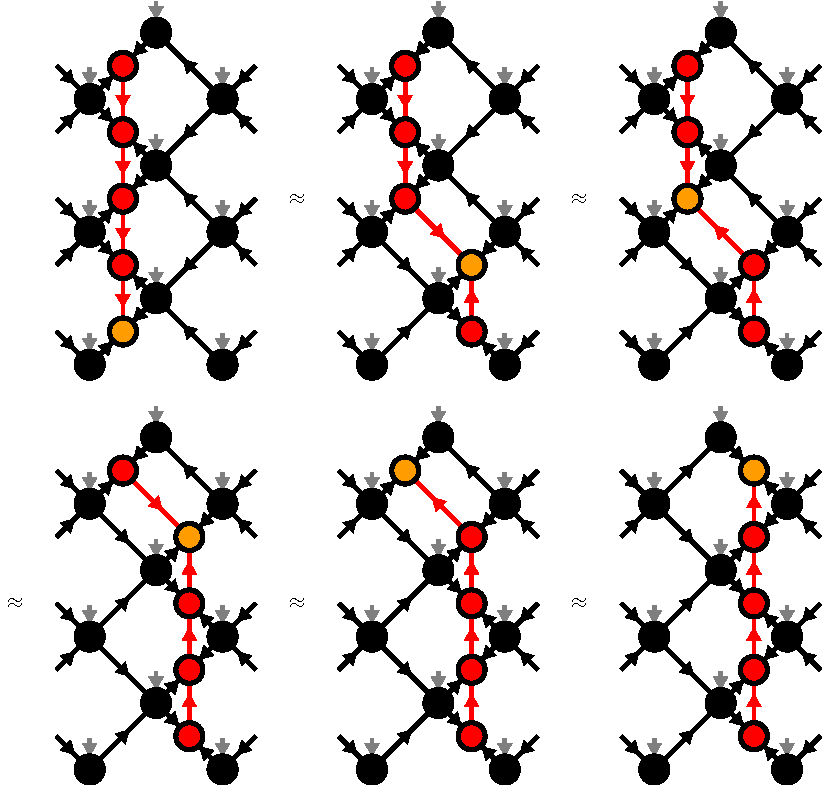
\includegraphics[scale=1]{figures/tikz/disoTPS/shifting_ortho_surface/shifting_ortho_surface.pdf}
	\caption{Two YB-moves are used to shift the orthogonality hypersurface one column to the right. In the last step, the orthogonality center can be moved across the $T$-tensor by contracting the two tensors and performing a truncated SVD.}
	\label{fig:disoTPS_moving_ortho_surface}
\end{figure}
Most algorithms implemented on disoTPS require an efficient procedure for moving the orthogonality surface, where the error introduced by this procedure should be as small as possible. For isoTPS, the current best procedure is given by the Moses Move, followed by an optional variational optimization. \par
In analogy to the MM we look for a procedure to iteratively shift the orthogonality surface through one column of $T$-tensors as shown in figure \figref{fig:disoTPS_moving_ortho_surface}. A single iteration of this process is shown in figure \figref{fig:disoTPS_YB_move_closeup}. The two tensors $W_1$ and $W_2$, which are part of the orthogonality hypersurface, are "pulled through" the site tensor $T$, resulting in the updated tensors $T^\prime$, $W_1^\prime$ and $W_2^\prime$. To keep the isometric structure of the network, $T^\prime$ and $W_1^\prime$ must be isometries, while $W_2^\prime$ must be a tensor of norm one (the new orthogonality center). Due to the visual similarity to the Yang-Baxter equation we call this procedure the \textit{Yang-Baxter} (YB) move. \par
We denote the state represented by the disoTPS before the YB move by $\left|\Psi\right\rangle = \left|\Psi\left(W_1, W_2, T\right)\right\rangle$ and the state after the YB move by $\left|\Psi^\prime\right\rangle = \left|\Psi^\prime\left(W_1^\prime, W_2^\prime, T^\prime\right)\right\rangle$. One can think of the YB move as an optimization problem
\begin{equation}
	\label{eq:disoTPS_YB_move_standard}
	\left(T^\prime_\text{opt},W_{1,\text{opt}}^\prime,W_{2,\text{opt}}^\prime\right) = \underset{T^\prime,W_1^\prime,W_2^\prime}{\argmin}\left\lVert \left|\Psi\right\rangle - \left|\Psi^\prime\right\rangle\right\rVert_\text{F}
\end{equation}
under the constraints
\begin{equation}
	\label{eq:disoTPS_YB_move_constraints}
	T^{\prime\dagger}T^\prime = \id, \quad W_1^{\prime\dagger}W_1^\prime = \id, \quad \left\lVert W_2^\prime \right\rVert_\text{F} = 1.
\end{equation}
One can rewrite the error of the YB move as
\begin{equation}
	\label{eq:disoTPS_YB_move_rewritten_error}
	\begin{split}
		\left\lVert \left|\Psi\right\rangle - \left|\Psi^\prime\right\rangle \right\rVert_\text{F} =& \sqrt{\left\langle\Psi\middle|\Psi\right\rangle + \left\langle\Psi^\prime\middle|\Psi^\prime\right\rangle - 2\Re\left\langle\Psi\middle|\Psi^\prime\right\rangle} \\
		=& \sqrt{2 - 2\Re\left\langle\Psi\middle|\Psi^\prime\right\rangle},
	\end{split}
\end{equation}
where in the second step we used the fact that the wave function is normalized to one, $\left\langle\Psi\middle|\Psi\right\rangle = \left\langle\Psi^\prime\middle|\Psi^\prime\right\rangle = 1$. It follows that the optimization problem of minimizing the error becomes the problem of maximizing the overlap
\begin{equation}
	\label{eq:disoTPS_YB_move_alternative_formulation}
	\left(T^\prime_\text{opt},W_{1,\text{opt}}^\prime,W_{2,\text{opt}}^\prime\right) = \underset{T^\prime,W_1^\prime,W_2^\prime}{\text{argmax}}\Re\left\langle\Psi\middle|\Psi^\prime\right\rangle
\end{equation}
under the constraints \eqref{eq:disoTPS_YB_move_constraints}. Because the only tensors that are changed by the YB move are $W_1$, $W_2$ and $T$ and the three tensors make up a subregion of the full network with only incoming arrows, we can use the isometry condition and the computation of the overlap $\langle\Psi|\Psi^\prime\rangle$ reduces to a contraction of only six tensors as shown in figure \figref{fig:YB_move_iterate_polar_overlap}.\par
\begin{figure}
	\centering
	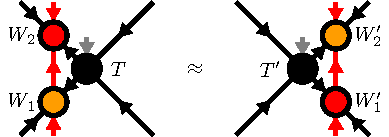
\includegraphics[scale=1]{figures/tikz/disoTPS/yang_baxter_move/yang_baxter_move.pdf}
	\caption{The Yang-Baxter (YB) move is the procedure of "pulling" two auxillary tensors $W_1$ and $W_2$ through a site tensor $T$.}
	\label{fig:disoTPS_YB_move_closeup}
\end{figure}
In the following, we present two explicit algorithms for performing the YB move. The first algorithm (see section \ref{sec:YB_move_iterative_local_optimization}) is an variational optimization method with iterative local updates. The second algorithm (see section \ref{sec:YB_move_svd_disentangle}) is a tripartite decomposition with disentangling similar to the tripartite decomposition used in the MM. In section \ref{sec:YB_move_comparison} we will compare the two algorithms.

\subsection{variational optimization with local updates}
\label{sec:YB_move_iterative_local_optimization}
To solve the constrained optimization problem \eqref{eq:YB_isoTPS_YB_move_alternative_formulation} we proceed by maximizing the overlap while only varying the parameters of one of the three tensors $T^\prime$, $W_1^\prime$ or $W_2^\prime$, treating all other tensors as constant. For example, let us keep $W_1^\prime$ and $W_2^\prime$ fixed and optimize $T^\prime$. We first contract all tensors except $T^\prime$ into an environment $E$ as shown in Figure \figref{fig:YB_move_iterate_polar_optimize_T}. We can then write the optimization problem as
\begin{equation}
	T^\prime_\text{opt} = \underset{T^{\prime\dagger}T = \id}{\argmax} \Re\braket{\Psi,\Psi^\prime} = \underset{T^{\prime\dagger}T = \id}{\argmax}\Re\left\langle E, T^\prime\right\rangle_\text{F} = \underset{T^{\prime\dagger}T = \id}{\argmax}\Re\Tr\left(T^{\prime\dagger}E\right).
\end{equation}
This problem is known as the \textit{orthogonal Procrustes problem} and permits the closed form solution $T^\prime_\text{opt} = UV^\dagger$, where $U$ and $V$ are computed using the SVD $E = USV^\dagger$. For the derivation of this solution see Appendix \ref{app:optimization_problems_for_isometric_tensor_networks}. The tensors $W_1^\prime$ and $W_2^\prime$ can be optimized similarly. The full algorithm is then performed by sweeping over the three tensors, optimizing them iteratively until convergence. Tensor diagrams for the algorithm are shown in Figure \figref{fig:YB_move_iterate_polar}. We discuss one iteration of the algorithm in more detail:
\begin{enumerate}
	\item Contract all tensors except $T^\prime$ into an environment $E$ and perform an SVD $E = USV$. The tensor $T^\prime$ is then updated as $T^\prime\leftarrow UV^\dagger$. See Figure \figref{fig:YB_move_iterate_polar_optimize_T}.
	\item Contract all tensors except $W_1^\prime$ into an environment $E$ and perform an SVD $E = USV$. The tensor $W_1^\prime$ is then updated as $W_1^\prime\leftarrow UV^\dagger$. See Figure \figref{fig:YB_move_iterate_polar_optimize_W1}.
	\item Contract all tensors except $W_2^\prime$ into an environment $E$. The tensor $W_1^\prime$ is then updated as $W_1^\prime\leftarrow E/\left\lVert E\right\rVert$. See Figure \figref{fig:YB_move_iterate_polar_optimize_W2}.
\end{enumerate}
These three steps are repeated until a termination criterion is met, for example until the decrease in error after one iteration is smaller than a given threshold or if a given maximum number of iterations $N_\text{iter}$ is exceeded. A similar algorithm was also used by Evenbly and Vidal in the context of the multi-scale entanglement renormalization ansatz
(MERA) \cite{cite:algorithms_for_entanglement_renormalization, cite:algorithms_for_entanglement_renormalization_boundaries_impurities_interfaces}. Note that in step three of the algorithm, a norm constraint is enforced instead of an isometry constraint, in which case the closed form solution takes a different shape. We also derive this solution in Appendix \ref{app:optimization_problems_for_isometric_tensor_networks}.\par
\begin{figure}
	\centering
	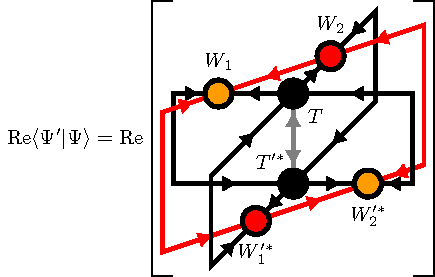
\includegraphics[scale=1]{figures/tikz/YB_isoTPS/yang_baxter_move_iterative/yang_baxter_move_iterative_a.pdf}
	\caption{The cost function of the optimization problem \eqref{eq:YB_isoTPS_YB_move_alternative_formulation} can be computed as a contraction of only six tensors.}
	\label{fig:YB_move_iterate_polar_overlap}
\end{figure}
\begin{figure}
	\centering
	\begin{subfigure}[c]{0.85\textwidth}
		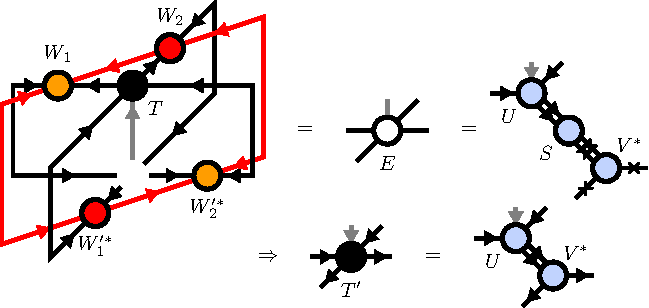
\includegraphics[scale=1]{figures/tikz/YB_isoTPS/yang_baxter_move_iterative/yang_baxter_move_iterative_b.pdf}
		\caption{}\label{fig:YB_move_iterate_polar_optimize_T}
	\end{subfigure}
	\begin{subfigure}[c]{0.85\textwidth}
		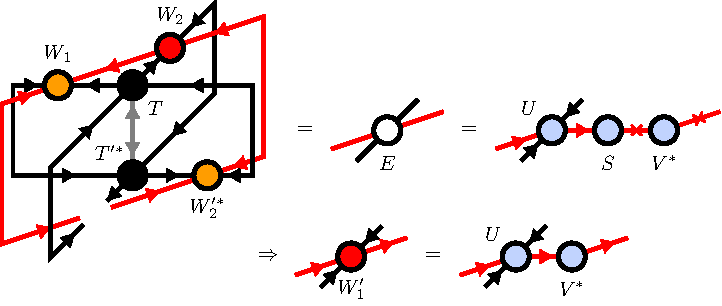
\includegraphics[scale=1]{figures/tikz/YB_isoTPS/yang_baxter_move_iterative/yang_baxter_move_iterative_c.pdf}
		\caption{}\label{fig:YB_move_iterate_polar_optimize_W1}
	\end{subfigure}
	\begin{subfigure}[c]{0.85\textwidth}
		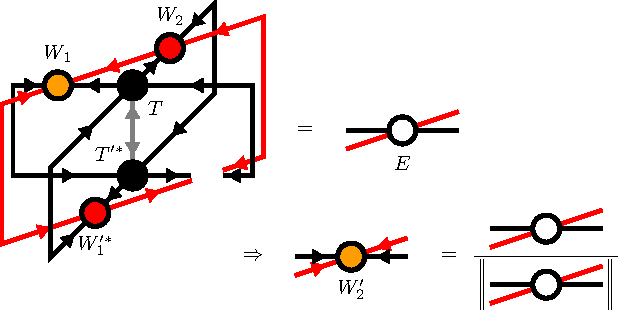
\includegraphics[scale=1]{figures/tikz/YB_isoTPS/yang_baxter_move_iterative/yang_baxter_move_iterative_d.pdf}
		\caption{}\label{fig:YB_move_iterate_polar_optimize_W2}
	\end{subfigure}%
	\caption{In this figure we show the three local updates that are used to iteratively solve optimization problem \eqref{eq:YB_isoTPS_YB_move_alternative_formulation}. (a) The tensor $T^\prime$ can be updated similarly by contracting all tensors except $T^\prime$ into the environment $E$ and isometrizing $E$ using an SVD. (b) The tensor $W_1^\prime$ can be updated by contracting all tensors except $W_1^\prime$ into the environment $E$, which is subsequently isometrized using an SVD. (c) To optimize the tensor $W_2^\prime$, all tensors except $W_2^\prime$ are contracted into the environment $E$. The updated tensor is then given as $W_2^\prime = E/\lVert E\rVert$.}
	\label{fig:YB_move_iterate_polar}
\end{figure}
The computational cost of the algorithm is dominated by the tensor contractions, scaling as $\mathcal{O}(3N_\text{iter}(\chi^2D^6d + \chi^3D^4)) = \mathcal{O}(N_\text{iter}D^8)$ for one YB move.\par
\begin{figure}
	\centering
	\begin{tikzpicture}[scale=1, trim axis left, trim axis right]
		\begin{axis}[xlabel=$N_\text{iters}$, ylabel={$\lVert|\Psi\rangle-|\Psi^\prime\rangle\rVert$}, grid=both, grid style={gray!20}, every axis plot/.append style={very thick}, scale only axis, height=\singleFigureHeight, width=\singleFigureWidth]
			
			\addplot[color = 5blue4]
			table[x=N_iter, y=trunc_error, col sep=space]{figures/plots/disoTPS/data/iterate_polar.txt};
			%\addlegendentry{Evenbly-Vidal}
			
		\end{axis}
	\end{tikzpicture}
	\caption{We show a cool figure here!!\todo{Caption}}
	\label{fig:disoTPS_tripartite_decomposition_iterate_polar}
\end{figure}
In practice we observe that the discussed algorithm converges only very slowly. To qualitatively showcase this, we perform the YB move on a typical environment of tensors $\left\{W_1, W_2, T\right\}$ that was encountered during imaginary time evolution of the Transverse Field Ising model, see Chapter \ref{chap:TFI} for more details. The bond dimensions chosen for the YB-isoTPS are $D = 4$, $\chi = 24$. We plot the error $\lVert\ket{\Psi}-\ket{\Psi^\prime}\rVert$ against the number of iterations in Figure \figref{fig:YB_isoTPS_tripartite_decomposition_iterate_polar}. After $N_\text{iter}=10000$ iterations, the algorithm is still not converged.

\subsection{Tripartite decompositon using an SVD and disentangling}
\label{sec:YB_move_svd_disentangle}
Alternatively, the constrained optimization problem \eqref{eq:disoTPS_YB_move_standard} can be solved via two successive SVDs with an optional disentangling prodcedure with the goal of reducing the truncation error or some entanglement measure. This is the same algorithm that was used for the MM in the original isoTPS \cite{cite:efficient_simulation_of_dynamics_in_two_dimensional_quantum_spin_systems}. The algorithm is sketched in figure \figref{} and is made up of three main steps.
\begin{enumerate}
	\item We start by contracting the tensors $T$, $W_1$ and $W_2$ into a single tensor $\Psi$ (figure \figref{} (b)). This tensor is then split from left to right via a truncated SVD
	\begin{equation}
		\Psi = XSZ^\dagger = X\left(SZ^\dagger\right) \eqqcolon X\theta
	\end{equation}
	as shown in figure \figref{}(c). The bond dimension is truncated to $D^2$.
	\item Next, we split the index of the bond connecting $X$ and $\theta$ into two indices of dimension $D$ each, see figure \figref{}(d). To proceed, we note that there exists a degree of freedom on the bonds connecting $X$ and $\theta$: A unitary $U$ and its adjoint can be inserted as shwon in figure \figref{}(e) without changing the result of the contraction
	\begin{equation}
		XU^\dagger U\theta = \left(XU^\dagger\right)\left(U\theta\right) \eqqcolon T^\prime \tilde{\theta}.
	\end{equation}
	This unitary $U$ can be chosen to minimize the truncation error of the next step by \textit{disentangling} the tensor $\theta$. We will discuss procedures of finding such a \textit{disentangling unitary} on the next page.
	\item In the last step, the tensor $\tilde{\theta}$ is split vertically into $W_1^\prime$ and $W_2^\prime$ using a truncated SVD as shown in figure \figref{}(f). Here, the bond dimension is truncated to $\chi$. We end up with the three tensors $T^\prime$, $W_1^\prime$ and $W_2^\prime$, completing the YB move.
\end{enumerate}
Before we discuss the disentangling procedure, two comments about step two of the above algorithm are in order. Firstly, there exists a degree of freedom for splitting the bond index, because applying the same permutations to the columns of $X$ and rows of $\theta$ does not change the result of contracting the network. Thus, there is no unique splitting that can be chosen. However, this degree of freedom is fixed by the disentangling process, making the exact permutation of the bond splitting irrelevant. Secondly, note that near the edges of the lattice it can happen that the matrizized tensor $\Psi$ has $\tilde{\chi} < D^2$ rows. In this case, the bond dimension after the SVD will also be $\tilde{\chi}$ and we cannot split the bond into two bonds of dimension $\chi_1=\chi_2=D$. Instead, we choose a splitting $\chi_1 \le D$, $\chi_2 \le D$ such that $\chi_1\cdot\chi_2$ is maximized while it must still hold $\chi_1\cdot\chi_2\le\tilde{\chi}$. We additionally prefer "equal" splittings $\chi_1\approx\chi_2\approx\sqrt{\tilde{\chi}}$ if possible. One can find such a splitting easily by computing all possible combinations of $\chi_1$ and $\chi_2$ and keeping only the best one. This has a computational cost of $\mathcal{O}\left(\sqrt{\tilde{\chi}}\right) = \mathcal{O}\left(d\right)$. \par
\begin{figure}
	%\includegraphics[width=0.8\textwidth]{figures/Tensor_Networks/yb_move_svd_disent.jpeg}
	\caption{test\todo{Why does this image not work? Also write caption.}}
	\label{fig:yb_move_svd_disent}
\end{figure}
We will now discuss the problem of finding a good disentangling unitary $U$ for step two of the above algorithm, which is crucial for the performance of the YB move. The problem can be formulated as follows: Given a tensor $\theta \in \mathbb{C}^{\chi_1\times d_1\times d_2\times \chi_2}$, find a unitary $U\in\mathbb{C}^{d_1\times d_2\times d_1\times d_2}$ minimizing a cost function
\begin{equation}
	f(\tilde{\theta}),
\end{equation}
where
\begin{equation}
	\tilde{\theta}\in\mathbb{C}^{\chi_1\times d_1\times d_2\times \chi_2}, \quad \tilde{\theta}_{\alpha,i,j,\beta} \coloneqq \sum_{i^\prime,j^\prime}U_{i,j,i^\prime,j^\prime}\theta_{\alpha,i,j,\beta}.
\end{equation}

\subsection{Comparison of the two algorithms}
\label{sec:YB_move_comparison}
\begin{figure}
	\centering
	\begin{tikzpicture}[scale=1, trim axis left, trim axis right]
		\begin{axis}[xlabel={walltime [s]}, ylabel={$\lVert|\Psi\rangle-|\Psi^\prime\rangle\rVert$}, grid=both, grid style={gray!20}, every axis plot/.append style={very thick}, scale only axis, height=\singleFigureHeight, width=\singleFigureWidth, xmode=log, legend pos=north east, legend style={nodes={scale=\legendscale, transform shape}}]
			%
			\addplot[color = blue]
			table[x=t, y=trunc_error, col sep=space]{figures/plots/disoTPS/data/comparing_tripartite_decompositions_iterate_polar.txt};
			\addlegendentry{EV trunc}
			%
			\addplot[color = red]
			table[x=t, y=trunc_error, col sep=space]{figures/plots/disoTPS/data/comparing_tripartite_decompositions_renyi_2_EV.txt};
			\addlegendentry{EV Rényi-$2$}
			%
			\addplot[color = 5orange4]
			table[x=t, y=trunc_error, col sep=space]{figures/plots/disoTPS/data/comparing_tripartite_decompositions_renyi_0.5_approx_trm.txt};
			\addlegendentry{appr.\,CG\,Rényi-$0.5$}
			%	
			\addplot[color = 5green4]
			table[x=t, y=trunc_error, col sep=space]{figures/plots/disoTPS/data/comparing_tripartite_decompositions_trunc_approx_trm.txt};
			\addlegendentry{appr. TRM trunc}
			%
		\end{axis}
	\end{tikzpicture}
	\caption{\todo{caption! + choose better colors in plot + better legend placement!}}
	\label{fig:yb_move_comparison}
\end{figure}

\section{Time Evolving Block Decimation (TEBD)}
\label{sec:YB_isoTPS_TEBD}
We will now discuss the Time Evolving Block Decimation (TEBD) algorithm for disoTPS, which can be used for both real and imaginary time evolution. The algorithm is a generalization of TEBD for MPS, which we discussed in Section \ref{sec:tensors_and_tensor_networks_matrix_product_states}. Analogously to MPS we start with a Suzuki-Trotter decomposition, approximating the time evolution operator $U\left(\Delta t\right) = e^{-i\Delta t \hat{H}}$ by a product of bond operators $U^{[x, y]}\left(\Delta t\right)$ acting only on neighbouring sites on the bond $[x, y]$. These bond operators then must be applied to the state in the correct order, while keeping the disoTPS structure intact. We will discuss the process of applying a single bond operator $U^{[x,y]}\left(\Delta t\right)$ to the disoTPS in Section \ref{sec:YB_isoTPS_TEBD_local_updates}. In Section \ref{sec:YB_isoTPS_TEBD_global_updates} we then discuss the full TEBD algorithm.

\subsection{Local TEBD updates}
\label{sec:YB_isoTPS_TEBD_local_updates}
\begin{figure}
	\centering
	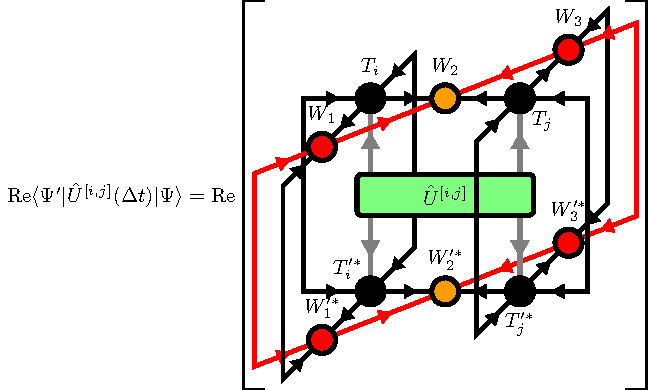
\includegraphics[scale=1]{figures/tikz/YB_isoTPS/tebd_environment/tebd_environment.pdf}
	\caption{The cost function of the optimization problem \eqref{eq:YB_isoTPS_TEBD_maximizing_overlap} that must be solved for locally applying TEBD operators $\hat{U}^{[i,j]} \coloneqq \hat{U}^{[i,j]}(\Delta t)$ can be computed as a contraction of the two-site wave functions of $\ket{\Psi}$ and $\ket{\Psi^\prime}$, sandwiching the operator between the two.}
	\label{fig:YB_isoTPS_TEBD_overlap_contraction}
\end{figure}
Let us assume that the orthogonality center is positioned between the two sites on which the bond operator $\hat{U}^{[x, y]}\left(\Delta t\right)$ acts. The five tensors around the orthogonality center then make up a sub-network with only incoming arrows, compare Figure \figref{fig:YB_isoTPS_twosite_expectation_value_environment}. We call these five tensors $T_1$, $T_2$, $W_1$, $W_2$ and $W_3$. The local TEBD update can then be formulated as the following problem: Find tensors $T_1^\prime$, $T_2^\prime$, $W_1^\prime$, $W_2^\prime$ and $W_3^\prime$ satisfying the isometry constraints and minimizing the error
\begin{equation}
	\label{eq:isoDTPS_TEBD_local_update_error}
	\varepsilon_\text{trunc} = \left\lVert \hat{U}^{[x,y]}(\Delta t)\ket{\Psi} - \ket{\Psi}\right\rVert
\end{equation}
Similar to the YB-move, we can rewrite this as the problem of maximizing the overlap
\begin{equation}
	\label{eq:YB_isoTPS_TEBD_maximizing_overlap}
	(T_{i,\text{opt}}^\prime, T_{j,\text{opt}}^\prime, W_{1,\text{opt}}^\prime, W_{2,\text{opt}}^\prime, W_{3,\text{opt}}^\prime)= \underset{T_i^\prime, T_j^\prime, W_1^\prime, W_2^\prime, W_3^\prime}{\argmax}\Re\bra{\Psi}\hat{U}^{[x,y]}(\Delta t)\ket{\Psi^\prime}.
\end{equation}
under the constraints $T_i^{\prime\dagger}T_i^\prime = \id$, $T_j^{\prime\dagger}T_j^\prime = \id$, $W_1^{\prime\dagger}W_1^\prime = \id$, $W_3^{\prime\dagger}T_3^\prime = \id$ and $\lVert W_2^\prime\rVert = 1$.
Using the isometry condition, the overlap $\bra{\Psi}\hat{U}^{[x,y]}(\Delta t)\ket{\Psi^\prime}$ can be computed by contracting the tensor network drawn in Figure \figref{fig:YB_isoTPS_TEBD_overlap_contraction}. For solving this problem we again use the Evenbly-Vidal algorithm. Similar to what we already did in Section \ref{sec:YB_move_iterative_local_optimization} for the YB move, we optimize one tensor at a time while keeping all other tensors fixed. This procedure is then repeated, sweeping over all five tensors until convergence is achieved. For more details on this optimization method see Appendix \ref{app:riemannian_optimization_of_isometries}. Since the time step $\Delta t$ is chosen to be small, the bond operator is close to identity, $\hat{U}^{[x,y]}(\Delta t)\approx\id$. Thus, a good initialization for the tensors of the updated wave function $\ket{\Psi^\prime}$ are simply the tensors of the old wave function $\ket{\Psi}$. \par
The computational complexity of applying a local bond operator to a disoTPS with the discussed algorithm scales as $\mathcal{O}(\chi^3D^3d^2) = \mathcal{O}(D^6)$. In practice it is observed that the algorithm converges after only a few iterations.

\subsection{Global TEBD updates}
\label{sec:YB_isoTPS_TEBD_global_updates}
\begin{figure}
	\centering
	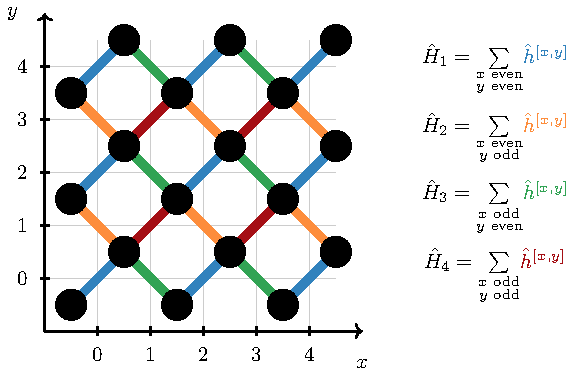
\includegraphics[scale=1]{figures/tikz/YB_isoTPS/tebd_global_update/tebd_global_update_a.pdf}
	\caption{A Hamiltonian $\hat{H}$ that is a sum of nearest-neighbour operators $h^{[x,y]}$ can be split into four parts made up of operators acting only on even/odd columns and even/odd bonds along a column.}
	\label{fig:YB_isoTPS_TEBD_global_update_TEBD1_splitting_and_TEBD2_chain}
\end{figure}
A global TEBD update evolves the state by a time $\Delta t$ and can be performed by applying local TEBD updates on all bonds. For each local TEBD update, the orthogonality center must be moved to the bond at which the update is applied. Because moving the orthogonality hypersurface can only be done approximately, the number of necessary moves should be minimized. \par
As we have already done for MPS in Section \ref{sec:tensors_and_tensor_networks_matrix_product_states}, let us assume that the Hamiltonian $\hat{H}$ can be written as a sum of nearest-neighbour operators. We index these nearest-neighbour operators $h^{[x, y]}$ by two integers $x$ and $y$ corresponding to the position of the orthogonality hypersurface and orthogonality center if moved to the bond on which $h^{[x,y]}$ acts. We define $x$ to increase from left to right and $y$ to increase from bottom to top, as shown in Figure \figref{fig:YB_isoTPS_TEBD_global_update_TEBD1_splitting_and_TEBD2_chain}. The Hamiltonian can then be split into four parts by first grouping the $h^{[x,y]}$ into two sets acting only on even and odd columns respectively and then splitting each set again into terms acting only on even/odd bonds along the respective columns. We can write this as
\begin{equation}
	\label{eq:YB_isoTPS_TEBD_splitting_local_Hamiltonian}
	\begin{split}
		\hat{H} = \sum_{x=1}^{2L_x-1} \sum_{y=1}^{2L_y-1}h^{[x,y]} &= \sum_{\substack{x\text{ even}\\y\text{ even}}} h^{[x, y]} + \sum_{\substack{x\text{ even}\\y\text{ odd}}} h^{[x, y]} + \sum_{\substack{x\text{ odd}\\y\text{ even}}} h^{[x, y]} + \sum_{\substack{x\text{ odd}\\y\text{ odd}}} h^{[x, y]} \\
		&\eqqcolon \hat{H}_1 + \hat{H}_2 + \hat{H}_3 + \hat{H}_4.
	\end{split}
\end{equation}
The operators appearing in the sum in $\hat{H}_j$ commute with each other and thus the exponential $e^{-i\Delta t\hat{H}_j}$ factorizes into a product of bond operators $\hat{U}^{[x, y]}(\Delta t) = e^{-i\Delta t\hat{h}^{[x, y]}}$. \par
We next use a Suzuki-Trotter decomposition to approximate the time evolution operator
\begin{equation}
	\label{eq:YB_isoTPS_TEBD_suzuki_trotter_first_order}
	\hat{U}(\Delta t) = \hat{U}^\text{TEBD1}(\Delta t) + \mathcal{O}(\Delta t^2)
\end{equation}
with
\begin{equation}
	\label{eq:YB_isoTPS_TEBD_first_order_TEBD_operator}
	\hat{U}^\text{TEBD}(\Delta t) \coloneqq e^{-i\Delta t\hat{H}_4} e^{-i\Delta t\hat{H}_3} e^{-i\Delta t\hat{H}_2} e^{-i\Delta t\hat{H}_1}.
\end{equation}
To evolve the state $\ket{\Psi}$ in time with this first order approximation we must compute $\ket{\Psi^\prime} \approx U^\text{TEBD1}(\Delta t)\ket{\Psi}$ as a disoTPS. The procedure is sketched in Figure \figref{fig:YB_isoTPS_TEBD_global_update_applying_TEBD1}. We start in the left-most column and apply all bond operators that act on bonds along this column. The bond operators on the column are applied in a brick-wall fashion analogously to the MPS algorithm: First all even bonds are updated and then all odd bonds are updated. Local updates are computed using the algorithm discussed in Section \ref{sec:YB_isoTPS_TEBD_local_updates}. Next, we move the orthogonality hypersurface two columns to the right and again apply all bond operators along the column. We proceed until all bond operators on even columns have been applied, in which case the orthogonality hypersurface is now positioned at its right-most position. We now sweep back to the left, applying all bond operators acting on odd columns along the way. Arriving back at the left-most column, all bonds making up $\hat{U}^\text{TEBD1}(\Delta t)$ have been applied in the correct order and the state has been evolved by time $\Delta t$. \par
\begin{figure}
	\centering
	\subcaptionbox{\label{fig:YB_isoTPS_TEBD_global_update_applying_TEBD1}}
	{%
		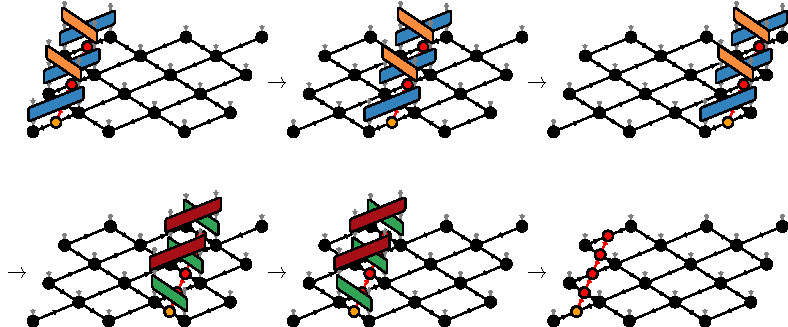
\includegraphics[scale=1]{figures/tikz/YB_isoTPS/tebd_global_update_steps/tebd_global_update_steps_a.pdf}
	}
	\par\bigskip\medskip
	\subcaptionbox{\label{fig:YB_isoTPS_TEBD_global_update_applying_TEBD2}}
	{%
		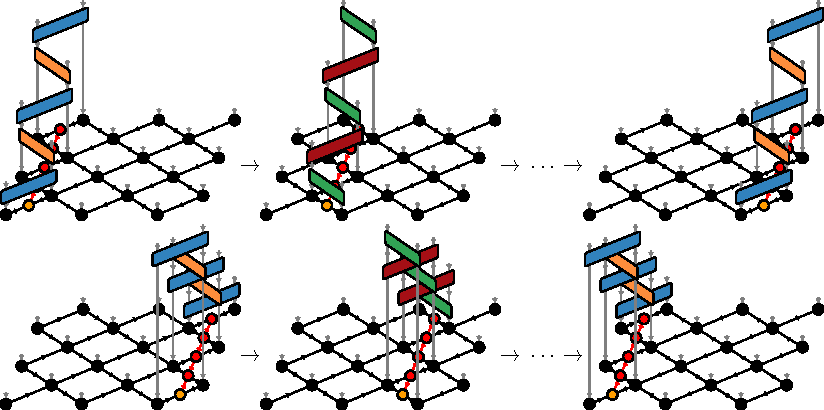
\includegraphics[scale=1]{figures/tikz/YB_isoTPS/tebd_global_update_steps/tebd_global_update_steps_b.pdf}
	}
	\caption{To apply a TEBD update, we sweep across the disoTPS once from left to right and back from right to left. (a) TEBD1 applies the operators in a brick-wall fashion, while (b) TEBD2 applies the operators along a chain.}
	\label{fig:YB_isoTPS_TEBD_global_update_applying_TEBD}
\end{figure}
We can obtain a better approximation of the time evolution operator $U(\Delta t)$ by performing a second order Suzuki-Trotter decomposition. By repeatedly applying the symmetrized decomposition
\begin{equation}
	e^{-i\varepsilon(A+B)} = e^{-i\frac{\varepsilon}{2}A}e^{-i\frac{\varepsilon}{2}A}e^{-i\varepsilon B} + \mathcal{O}(\Delta t^3)
\end{equation}
we obtain
\begin{equation}
	\begin{split}
		\label{eq:YB_isoTPS_tebd_second_order_suzuki_trotter_decomposition}
		e^{-i\Delta t\hat{H}} &= \exp\left(-i\Delta t\sum_{x,y}\hat{h}^{[x,y]}\right) \\
		&= e^{-i\frac{\Delta t}{2}\hat{h}^{[1, 1]}} e^{-i\Delta t\left(\hat{H}-\hat{h}^{[1,1]}\right)} e^{-i\frac{\Delta t}{2}\hat{h}^{[1, 1]}} + \mathcal{O}(\Delta t^3)\\
		&= e^{-i\frac{\Delta t}{2}\hat{h}^{[1, 1]}} e^{-i\frac{\Delta t}{2}\hat{h}^{[1, 2]}} e^{-i\Delta t\left(\hat{H}-\hat{h}^{[1,1]}-\hat{h}^{[1, 2]}\right)} e^{-i\frac{\Delta t}{2}\hat{h}^{[1, 2]}} e^{-i\frac{\Delta t}{2}\hat{h}^{[1, 1]}} + \mathcal{O}(\Delta t^3)\\
		&=\cdots\\
		&= e^{-i\frac{\Delta t}{2}\hat{h}^{[1, 1]}} e^{-i\frac{\Delta t}{2}\hat{h}^{[1, 2]}} \cdots e^{-i\frac{\Delta t}{2}\hat{h}^{[1, 2]}} e^{-i\frac{\Delta t}{2}\hat{h}^{[1, 1]}} + \mathcal{O}(\Delta t^3).
	\end{split}
\end{equation}
Here, in each step we "split off" one operator $\hat{h}^{[x,y]}$ from the sum. The final result is a product of bond operators $\hat{U}^{[x,y]}(\Delta t/2))$ that must be applied from right to left. The algorithm of applying a global second order update is thus similar to a TEBD update of first order. We sweep across the disoTPS once from left to right and back, applying bond operators along the way in the correct order, as visualized in Figure \figref{fig:YB_isoTPS_TEBD_global_update_applying_TEBD2}. The difference to TEBD1 is that now the operators are applied in a chain-like order instead of the brick wall order of TEBD1. The number of YB moves for TEBD1 and TEBD2 is the same, but the smaller Trotter error of $\mathcal{O}(\Delta t^3)$ instead of $\mathcal{O}(\Delta t^2)$ allows us to use larger time steps for TEBD2, resulting in a smaller number of YB moves per unit time. We find that the YB move is the primary source of error in practice and thus expect TEBD2 to perform much better than TEBD1. \par 
In principle, one could also go to higher decomposition orders \cite{cite:finding_exponential_product_formulas_of_higher_orders}. However, already a third order decomposition would necessitate a larger number of sweeps for applying the full update, increasing the error accumulated through YB moves. It is therefore not clear if higher order decompositions would be able to improve the method further.
